\documentclass[xcolor={table}]{beamer}
\mode<presentation>{
  \usetheme{Boadilla}
  \usefonttheme[onlylarge]{structurebold}
  \usefonttheme[stillsansseriflarge]{serif}
  \setbeamerfont*{frametitle}{size=\normalsize,series=\bfseries}
  % \setbeamertemplate{navigation symbols}{}
  \setbeamercovered{transparent}
}
\usepackage[english]{babel}
\usepackage[latin1]{inputenc}
\usepackage{times}
\usepackage[T1]{fontenc}
\usepackage{amsmath}
\usepackage{amssymb}
\usepackage{esint}
\usepackage{hyperref}
\usepackage{tikz}
\usepackage{xkeyval}
\usepackage{xargs}
\usepackage{verbatim}
\usepackage{listings}
\usepackage{multimedia}
\newcommand\hmmax{0}
\newcommand\bmmax{0}
\usepackage{bm}
\usepackage{siunitx}
\usepackage{xcolor,pifont}

\usetikzlibrary{
  arrows,
  calc,
  decorations.pathmorphing,
  decorations.pathreplacing,
  decorations.markings,
  fadings,
  positioning,
  shapes,
  arrows.meta
}
\usepgfmodule{oo}

\pgfdeclareradialshading{glow2}{\pgfpoint{0cm}{0cm}}{
  color(0mm)=(white);
  color(2mm)=(white);
  color(8mm)=(black);
  color(10mm)=(black)
}
\pgfdeclareradialshading{glow}{\pgfpoint{0cm}{0cm}}{
  color(0mm)=(white);
  color(5mm)=(white);
  color(9mm)=(black);
  color(10mm)=(black)
}

\begin{tikzfadingfrompicture}[name=glow fading]
  \shade [shading=glow] (0,0) circle (1);
\end{tikzfadingfrompicture}

\begin{tikzfadingfrompicture}[name=glow2 fading]
  \shade [shading=glow2] (0,0) circle (1);
\end{tikzfadingfrompicture}

\mode<handout>{
  \usepackage{pgfpages}
  \pgfpagesuselayout{4 on 1}[a4paper,landscape,border shrink=5mm]
  \setbeamercolor{background canvas}{bg=black!10}
}

\newcommand\pgfmathsinandcos[3]{%
  \pgfmathsetmacro#1{sin(#3)}%
  \pgfmathsetmacro#2{cos(#3)}%
}
\newcommand\LongitudePlane[3][current plane]{%
  \pgfmathsinandcos\sinEl\cosEl{#2} % elevation
  \pgfmathsinandcos\sint\cost{#3} % azimuth
  \tikzset{#1/.estyle={cm={\cost,\sint*\sinEl,0,\cosEl,(0,0)}}}
}
\newcommand\LatitudePlane[3][current plane]{%
  \pgfmathsinandcos\sinEl\cosEl{#2} % elevation
  \pgfmathsinandcos\sint\cost{#3} % latitude
  \pgfmathsetmacro\yshift{\cosEl*\sint}
  \tikzset{#1/.estyle={cm={\cost,0,0,\cost*\sinEl,(0,\yshift)}}} %
}
\newcommand\DrawLongitudeCircle[2][1]{
  \LongitudePlane{\angEl}{#2}
  \tikzset{current plane/.prefix style={scale=#1}}
  % angle of "visibility"
  \pgfmathsetmacro\angVis{atan(sin(#2)*cos(\angEl)/sin(\angEl))} %
  \draw[current plane] (\angVis:1) arc (\angVis:\angVis+180:1);
  \draw[current plane,dashed] (\angVis-180:1) arc (\angVis-180:\angVis:1);
}
\newcommand\DrawLatitudeCircleArrow[2][1]{
  \LatitudePlane{\angEl}{#2}
  \tikzset{current plane/.prefix style={scale=#1}}
  \pgfmathsetmacro\sinVis{sin(#2)/cos(#2)*sin(\angEl)/cos(\angEl)}
  % angle of "visibility"
  \pgfmathsetmacro\angVis{asin(min(1,max(\sinVis,-1)))}
  \draw[current plane,decoration={markings, mark=at position 0.6 with {\arrow{<}}},postaction={decorate},line width=.6mm] (\angVis:1) arc (\angVis:-\angVis-180:1);
  \draw[current plane,dashed,line width=.6mm] (180-\angVis:1) arc (180-\angVis:\angVis:1);
}
\newcommand\DrawLatitudeCircle[2][1]{
  \LatitudePlane{\angEl}{#2}
  \tikzset{current plane/.prefix style={scale=#1}}
  \pgfmathsetmacro\sinVis{sin(#2)/cos(#2)*sin(\angEl)/cos(\angEl)}
  % angle of "visibility"
  \pgfmathsetmacro\angVis{asin(min(1,max(\sinVis,-1)))}
  \draw[current plane] (\angVis:1) arc (\angVis:-\angVis-180:1);
  \draw[current plane,dashed] (180-\angVis:1) arc (180-\angVis:\angVis:1);
}
\newcommand\coil[1]{
  {\rh * cos(\t * pi r)}, {\apart * (2 * #1 + \t) + \rv * sin(\t * pi r)}
}
\makeatletter
\define@key{DrawFromCenter}{style}[{->}]{
  \tikzset{DrawFromCenterPlane/.style={#1}}
}
\define@key{DrawFromCenter}{r}[1]{
  \def\@R{#1}
}
\define@key{DrawFromCenter}{center}[(0, 0)]{
  \def\@Center{#1}
}
\define@key{DrawFromCenter}{theta}[0]{
  \def\@Theta{#1}
}
\define@key{DrawFromCenter}{phi}[0]{
  \def\@Phi{#1}
}
\presetkeys{DrawFromCenter}{style, r, center, theta, phi}{}
\newcommand*\DrawFromCenter[1][]{
  \setkeys{DrawFromCenter}{#1}{
    \pgfmathsinandcos\sint\cost{\@Theta}
    \pgfmathsinandcos\sinp\cosp{\@Phi}
    \pgfmathsinandcos\sinA\cosA{\angEl}
    \pgfmathsetmacro\DX{\@R*\cost*\cosp}
    \pgfmathsetmacro\DY{\@R*(\cost*\sinp*\sinA+\sint*\cosA)}
    \draw[DrawFromCenterPlane] \@Center -- ++(\DX, \DY);
  }
}
\newcommand*\DrawFromCenterText[2][]{
  \setkeys{DrawFromCenter}{#1}{
    \pgfmathsinandcos\sint\cost{\@Theta}
    \pgfmathsinandcos\sinp\cosp{\@Phi}
    \pgfmathsinandcos\sinA\cosA{\angEl}
    \pgfmathsetmacro\DX{\@R*\cost*\cosp}
    \pgfmathsetmacro\DY{\@R*(\cost*\sinp*\sinA+\sint*\cosA)}
    \draw[DrawFromCenterPlane] \@Center -- ++(\DX, \DY) node {#2};
  }
}
\makeatother

% not mandatory, but I though it was better to set it blank
\setbeamertemplate{headline}{}
\def\beamer@entrycode{\vspace{-\headheight}}

\tikzstyle{snakearrow} = [decorate, decoration={pre length=0.2cm,
  post length=0.2cm, snake, amplitude=.4mm,
  segment length=2mm},thick, ->]

%% document-wide tikz options and styles

\tikzset{%
  % >=latex, % option for nice arrows
  inner sep=0pt,%
  outer sep=2pt,%
  mark coordinate/.style={inner sep=0pt,outer sep=0pt,minimum size=3pt,
    fill=black,circle}%
}
\tikzset{
  % Define standard arrow tip
  >=stealth',
  % Define style for boxes
  punkt/.style={
    rectangle,
    rounded corners,
    draw=black, very thick,
    text width=8em,
    minimum height=2.5em,
    text centered},
}

\tikzset{onslide/.code args={<#1>#2}{%
    \only<#1>{\pgfkeysalso{#2}}
    % \pgfkeysalso doesn't change the path
  }}
\tikzset{alt/.code args={<#1>#2#3}{%
    \alt<#1>{\pgfkeysalso{#2}}{\pgfkeysalso{#3}}
    % \pgfkeysalso doesn't change the path
  }}
\tikzset{temporal/.code args={<#1>#2#3#4}{%
    \temporal<#1>{\pgfkeysalso{#2}}{\pgfkeysalso{#3}}{\pgfkeysalso{#4}}
    % \pgfkeysalso doesn't change the path
  }}

\makeatletter
\newbox\@backgroundblock
\newenvironment{backgroundblock}[2]{%
  \global\setbox\@backgroundblock=\vbox\bgroup%
  \unvbox\@backgroundblock%
  \vbox to0pt\bgroup\vskip#2\hbox to0pt\bgroup\hskip#1\relax%
}{\egroup\egroup\egroup}
\addtobeamertemplate{background}{\box\@backgroundblock}{}
\makeatother

% \def\timeleft{15:00->14:55}

\title[Detecting leakage error]{Protecting quantum entanglement from leakage and qubit errors via repetitive parity measurements}
\date{Aug. 24, 2020}
\author{Yichao Yu}
\institute{Ni Group}

\ifpdf
% Ensure reproducible output
\pdfinfoomitdate=1
\pdfsuppressptexinfo=-1
\pdftrailerid{}
\hypersetup{
  pdfcreator={},
  pdfproducer={}
}
\fi

\begin{document}

\begin{frame}{}
  \titlepage
\end{frame}

\begin{frame}{Leakage}
  \begin{center}
    \textbf{Transition to outside the qubit space}\\
    \begin{columns}
      \column{8cm}
      \begin{itemize}
      \item<2-> Detection of leakage error
      \item<3-> Detection fidelity
      \item<4-> Correction of leakage error
      \end{itemize}
    \end{columns}
  \end{center}
\end{frame}

\begin{frame}{Setup}
  \begin{center}
    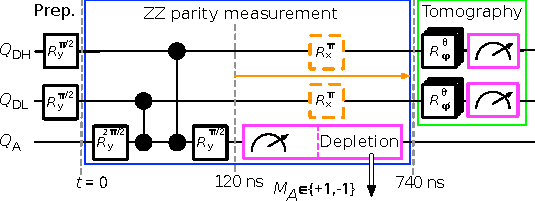
\includegraphics[width=8cm]{setup1}
    \begin{columns}
      \column{10cm}
      \begin{itemize}
      \item<2-> $Q_{DH}$, $Q_{DL}$, $Q_{A}$
      \item<3-> Error correction via post-processing\\
        \uncover<-2,4->{Requires symmetry between states}
      \item<5->$Z\otimes Z$ (and $X\otimes X$)
      \item<6->$F_{|\Psi^+\rangle|M_A={\pm1}}$, i.e. $P(Z\otimes Z=\pm1)$.
      \item<7->$F_{|\Psi^+\rangle}$, i.e. $P(|\Psi^+\rangle)$, i.e. $P(Z\otimes Z=1\ \&\ X\otimes X=1)$
      \end{itemize}
    \end{columns}
  \end{center}
\end{frame}

\begin{frame}{Repeated $Z$ measurement}
  \begin{center}
    \begin{columns}
      \column{6cm}
      \begin{center}
        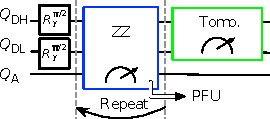
\includegraphics[width=4cm]{repeat_z}\\\vspace{0.2cm}
        \uncover<2->{
          \scriptsize{$Z\otimes Z\!=\!1$: $M_A\!=\!Const$}\\\vspace{0.2cm}
          \scriptsize{$Z\otimes Z\!=\!-1$: $M_A^{m}\!=\!-M_A^{m-1}$}
        }
      \end{center}
      \column{6cm}
      \begin{center}
        \visible<3->{
          \only<-3>{
            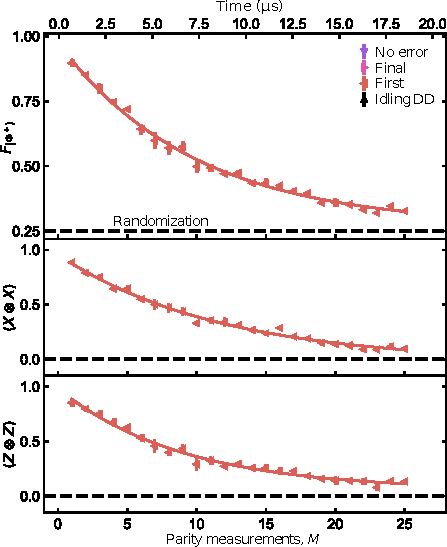
\includegraphics[width=6cm]{fidelity_z_first}
          }
          \only<4>{
            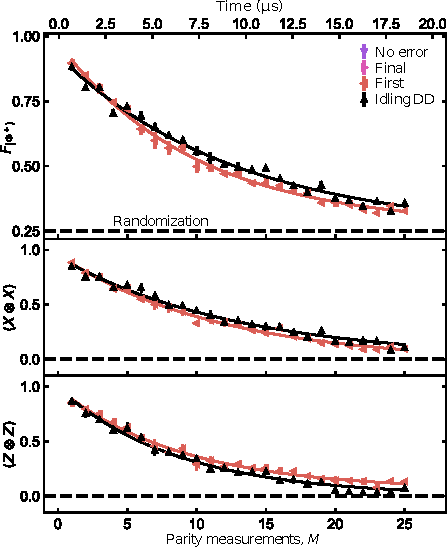
\includegraphics[width=6cm]{fidelity_z_idle_first}
          }
          \only<5>{
            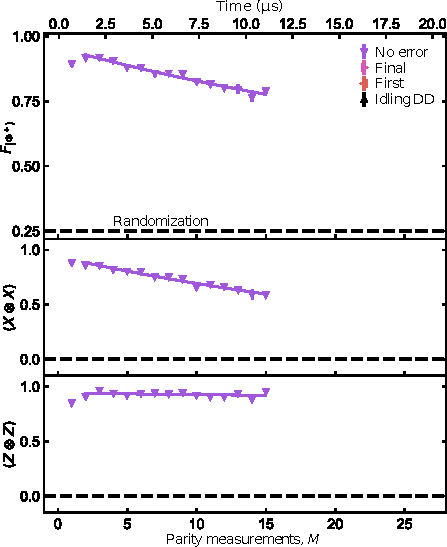
\includegraphics[width=6cm]{fidelity_z_noerror}
          }
          \only<6>{
            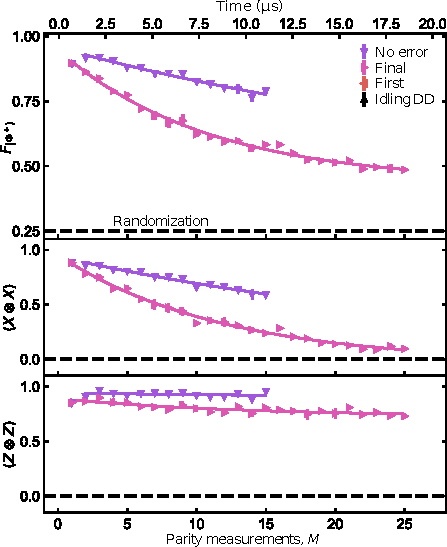
\includegraphics[width=6cm]{fidelity_z_final_noerror}
          }
        }
      \end{center}
    \end{columns}
  \end{center}
\end{frame}

\begin{frame}{Leakage detection and correction}
  \vspace{-0.9cm}
  \begin{center}
    \begin{columns}
      \column{6cm}
      \begin{center}
        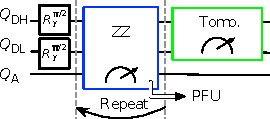
\includegraphics[width=4cm]{repeat_z}\\\vspace{0.4cm}
        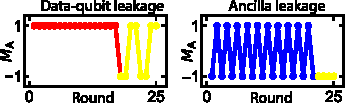
\includegraphics[width=5cm]{leak_types}\\\vspace{0.6cm}
        \visible<2->{
          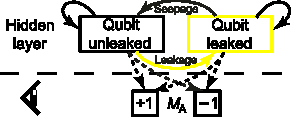
\includegraphics[width=5cm]{hmm}
        }
      \end{center}
      \column{6cm}
      \begin{center}
        \visible<3->{
          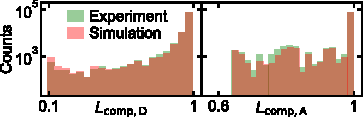
\includegraphics[width=5.5cm]{hmm_fit}\\\vspace{0.6cm}
        }
        \visible<4->{
          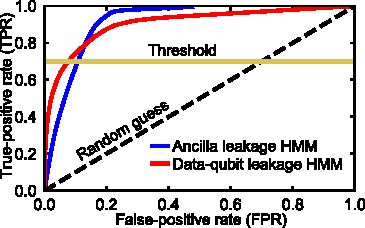
\includegraphics[width=5cm]{rocs}\\\vspace{0.6cm}
        }
        \visible<5->{
          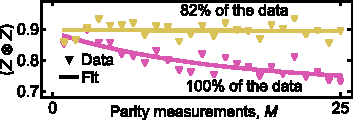
\includegraphics[width=5.5cm]{leak_correction}
        }
      \end{center}
    \end{columns}
  \end{center}
\end{frame}

\begin{frame}{Repeated $Z$ and $X$ measurement}
  \vspace{-0.9cm}
  \begin{center}
    \begin{columns}
      \column{4.5cm}
      \begin{center}
        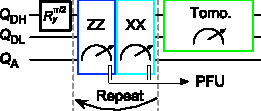
\includegraphics[width=4.5cm]{repeat_zx}
      \end{center}
      \column{7.5cm}
      \begin{center}
        \visible<2->{
          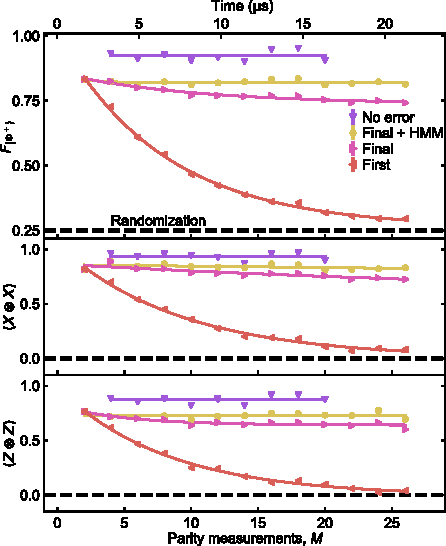
\includegraphics[width=6.5cm]{fidelity_zx}
        }
      \end{center}
    \end{columns}
  \end{center}
\end{frame}

\begin{frame}{Conclusion}
  \begin{center}
    \begin{columns}
      \column{8cm}
      \begin{itemize}
      \item Detection of leakage error\visible<2->{\hspace{0.1cm}\textcolor{green}{\ding{52}}}
      \item Detection fidelity\visible<3->{\hspace{0.1cm}\textcolor{orange}{\ding{52}\ $\approx90\%$}}
      \item Correction of leakage error\visible<4->{\hspace{0.1cm}\textcolor{red}{\ding{52}\ post selection}}
      \end{itemize}
    \end{columns}
  \end{center}
\end{frame}

\end{document}
